% Created 2026-11-19 Thu 12:28
% Intended LaTeX compiler: pdflatex
\documentclass[a4paper,11pt]{article}
\usepackage[utf8]{inputenc}
\usepackage[T1]{fontenc}
\usepackage{graphicx}
\usepackage{longtable}
\usepackage{wrapfig}
\usepackage{rotating}
\usepackage[normalem]{ulem}
\usepackage{amsmath}
\usepackage{amssymb}
\usepackage{capt-of}
\usepackage{hyperref}
% --- Document metadata (must precede bv.sty which uses them in \hypersetup) ---
\newcommand{\bvReferenceNumber}{XXXXXX}
\newcommand{\bvIssue}{Pre}
\newcommand{\bvTitle}{Speed Strategies, Ocean Current and Fuel Cap -- Rotterdam--Gothenburg}
\newcommand{\bvDate}{\today}
\newcommand{\bvType}{Technical Note}
\newcommand{\bvAuthor}{Frode Bloch}
\newcommand{\bvCompany}{Brunvoll AS}
\newcommand{\bvClassification}{CONFIDENTIAL}
\usepackage{/home/blofro/src/rdt_analysis/bv}
\usepackage{siunitx}
\sisetup{per-mode=symbol, inter-unit-product=\ensuremath{\cdot}}
\DeclareSIUnit{\knot}{kn}
\usepackage{amsmath}
\author{Frode Bloch}
\date{\today}
\title{}
\hypersetup{
 pdfauthor={Frode Bloch},
 pdftitle={},
 pdfkeywords={},
 pdfsubject={},
 pdfcreator={Emacs 29.3 (Org mode 9.6.15)}, 
 pdflang={English}}
\begin{document}

\bvMainTitlePage
\tableofcontents
\newpage

\section{Introduction}
\label{sec:org996338f}

A ship owner has asked for a maximum fuel flow limit (fuel cap) in the
Propulsion Optimiser.  This note examines whether a fuel cap saves fuel
compared with the speed control function, when the vessel must arrive
at a fixed time.  It also quantifies the potential of speed profiles
planned with knowledge of current and weather, and summarises the
general fuel effect of speed variation and early arrival.

\section{Simulation}
\label{sec:org7b602a5}

\subsection{Route and vessel}
\label{sec:orgc775a70}

\begin{itemize}
\item Route Rotterdam Europoort -- Gothenburg (509 nm, 7 legs), both
directions, one departure per day through 2024 (about 360 voyages
per direction).
\item Nominal speed 10 kn; every strategy arrives at the scheduled time
(about 51 h).
\item Vessel model as in the earlier voyage studies for this route: hull
model test data, Wageningen C4 propeller with the Propulsion Optimiser
choosing pitch and rpm, MAN L27/38 engine map, Flettner rotor
(H = 28 m, D = 4 m, spin ratio 3; spun only when it improves thrust
over the stopped rotor).  The rotor's electric drive motor is assumed
supplied by an auxiliary generator at 215 g/kWh, and this fuel is
included in the voyage fuel.  No shaft generator load.
\end{itemize}

\subsection{Environment}
\label{sec:org74631ae}

\begin{itemize}
\item Waves and wind: NORA3 hindcast (MET Norway), hourly.  Wave added
resistance from strip theory, hull wind resistance from Blendermann
coefficients.
\item Current: Copernicus Marine Service North-West European Shelf physics
reanalysis, hourly surface current at about 7 km resolution, tides
included (product ID in Section 6).  The mean along-track current
magnitude was 0.37--0.38 kn, strongest off the Dutch coast (95th
percentile about 1.7 kn).
\end{itemize}

\subsection{Method}
\label{sec:org2815e09}

\begin{itemize}
\item The route is divided into about 100 segments of 5 nm.  For each
segment the fuel rate is computed as a function of speed through
water from calm-water resistance, waves, wind and rotor thrust, using
the optimiser's minimum-fuel pitch and rpm.
\item Only the along-track current component is used; the drift angle from
cross current is ignored.
\item Weather and current at each segment are taken at the scheduled time;
the strategies reach a segment within a few minutes of each other.
\item Each voyage's fuel is corrected to the exact scheduled arrival time.
\end{itemize}

\subsection{Strategies}
\label{sec:orgdbf5ac0}

All strategies arrive at the same time.

\begin{center}
\small
\begin{tabular}{p{4.2cm}p{10.4cm}}
Strategy & Description\\[0pt]
\hline
Constant SOG (speed control) & Reference: constant speed over ground\\[0pt]
Constant STW & Constant speed through water (approximately constant power)\\[0pt]
Optimised, current known & Speed profile minimising fuel with known current, calm-water fuel model\\[0pt]
Optimised, current + weather & Speed profile minimising fuel with known current, waves and wind\\[0pt]
Fuel cap \(k\times\) & Speed control, with speed reduced where the fuel rate would exceed \(k\) times the calm-water fuel rate at 10 kn; the lost time is made up by a uniformly higher speed elsewhere\\[0pt]
\end{tabular}
\end{center}

\section{Results}
\label{sec:orgab4cffe}

Fuel relative to constant speed over ground (speed control), same
arrival time, with the Flettner rotor.  Values in brackets are the same
simulation without the rotor.  Cap results exclude voyages where the
cap made the schedule impossible.

\begin{center}
\small
\begin{tabular}{p{5.6cm}p{2.6cm}p{2.6cm}p{3.2cm}}
Strategy & Rotterdam to Gothenburg & Gothenburg to Rotterdam & Voyages where schedule cannot be met\\[0pt]
\hline
Constant SOG (speed control) & 0 & 0 & --\\[0pt]
Constant STW & +0.04 \% (+0.10) & +0.04 \% (+0.10) & --\\[0pt]
Optimised, current known & -0.14 \% (-0.12) & -0.17 \% (-0.13) & --\\[0pt]
Optimised, current + weather known & \textbf{-0.58 \%} (-0.19) & \textbf{-0.63 \%} (-0.19) & --\\[0pt]
Fuel cap 1.1\(\times\) & +0.09 \% (-0.01) & +0.11 \% (-0.03) & 136 / 92 of about 360\\[0pt]
Fuel cap 1.2\(\times\) & +0.09 \% (+0.09) & +0.18 \% (+0.01) & 76 / 42\\[0pt]
Fuel cap 1.3\(\times\) & +0.12 \% (+0.07) & +0.16 \% (+0.05) & 45 / 23\\[0pt]
Fuel cap 1.5\(\times\) & +0.16 \% (+0.09) & +0.12 \% (+0.10) & 16 / 7\\[0pt]
\end{tabular}
\end{center}

Observations:
\begin{itemize}
\item A fuel cap does not save fuel at a fixed arrival time; it costs
0.1--0.2 \% compared with speed control.  The cap slows the vessel
wherever the fuel rate is high, including in head current where the
optimum is to speed up, and the lost time is made up where speed is
not particularly cheap.
\item A tight cap makes the schedule impossible in heavy weather on a large
share of voyages (more than one third at 1.1\(\times\)).
\item Planning the speed with knowledge of current alone gains about
0.15 \%.  With the Flettner rotor, planning with current and weather
gains about 0.6 \% on average, and 1--1.4 \% on the 10 \% most
favourable voyages: the optimum sails faster when the rotor is
effective and slower in head wind.
\item A fuel cap may still be wanted for other purposes, such as limiting
engine load, staying within a consumption budget, or deliberately
accepting later arrival in bad weather.
\end{itemize}

\section{Speed control saving potential}
\label{sec:org86e0329}

The examples below are for a 240 nm leg scheduled for 24 h at an
average speed of 10 kn.  The fuel rate is assumed proportional to
\(V^3\).  At higher speeds the exponent increases (wave-making resistance,
engine load), so the larger deviations are somewhat underestimated.

\subsection{Speed variation at equal arrival time}
\label{sec:org3db0955}

The vessel sails above the setpoint for part of the leg and slower for
the rest, arriving at the scheduled time.

\begin{center}
\begin{tabular}{llll}
Deviation & +1 kn & +2 kn & +3 kn\\[0pt]
\hline
1 h above setpoint & +0.13 \% & +0.56 \% & +1.29 \%\\[0pt]
3 h above setpoint & +0.44 \% & +1.81 \% & +4.19 \%\\[0pt]
\end{tabular}
\end{center}

For random speed variation with standard deviation \(\sigma\) around the
average, the extra fuel is \(3\sigma^2/\bar{V}^2\):

\begin{center}
\begin{tabular}{lllll}
\(\sigma\) & 0.3 kn & 0.5 kn & 1 kn & 2 kn\\[0pt]
\hline
Extra fuel & +0.27 \% & +0.75 \% & +3.0 \% & +12 \%\\[0pt]
\end{tabular}
\end{center}

The penalty grows with the square of the deviation.  Normal speed
variations cost a few tenths of a percent.

\begin{figure}[htbp]
\centering
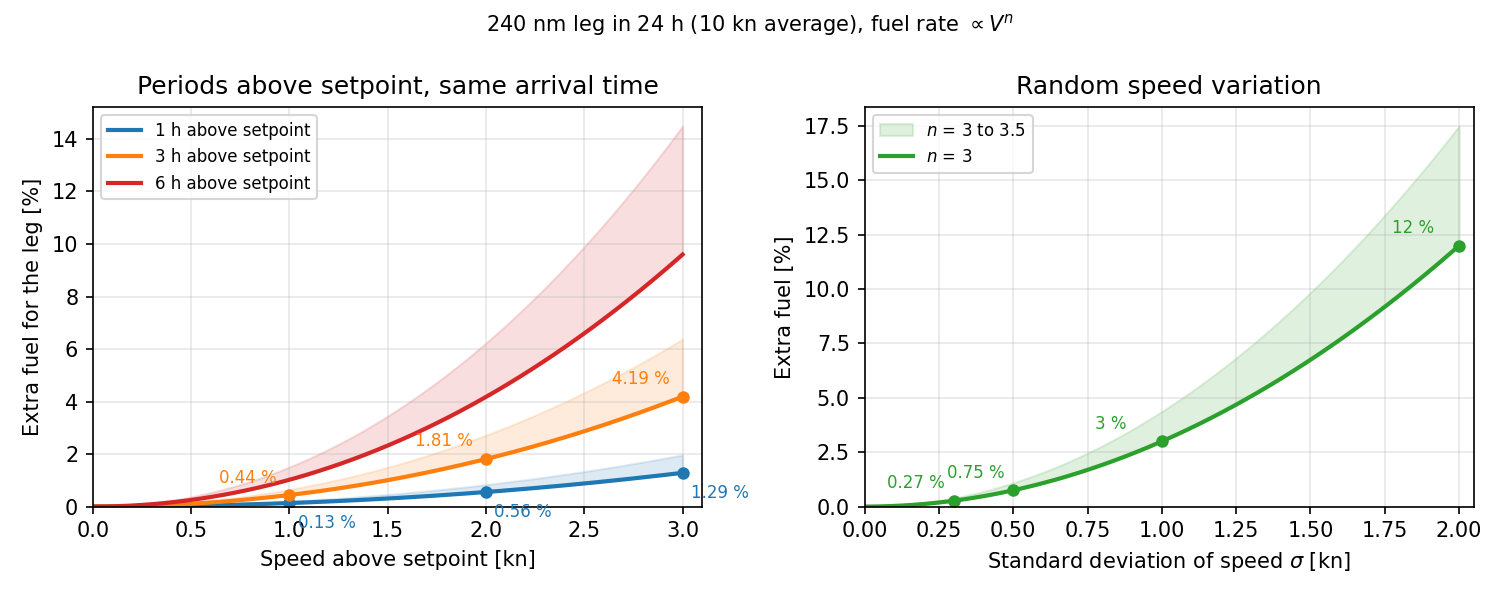
\includegraphics[width=\textwidth]{images/speed_variation_penalty.png}
\caption{Extra fuel from speed variation at equal arrival time.  Left: periods above the setpoint.  Right: random variation.  The bands show fuel rate exponents \(n\) = 3 to 3.5.}
\end{figure}

\subsection{Arriving early}
\label{sec:org37ed91e}

Arriving early means a higher average speed than required.  The fuel
for the leg is proportional to \(V^2\).  Fuel while waiting is not
included.

\begin{center}
\begin{tabular}{lll}
Arrives early by & Average speed & Extra fuel for the leg\\[0pt]
\hline
15 min & 10.11 kn & +2.1 \%\\[0pt]
30 min & 10.21 kn & +4.3 \%\\[0pt]
1 h & 10.43 kn & +8.9 \%\\[0pt]
2 h & 10.91 kn & +19 \%\\[0pt]
\end{tabular}
\end{center}

Arriving only 15 minutes early costs as much as sailing 3 h at 2.2 kn
above the setpoint.

\begin{figure}[htbp]
\centering
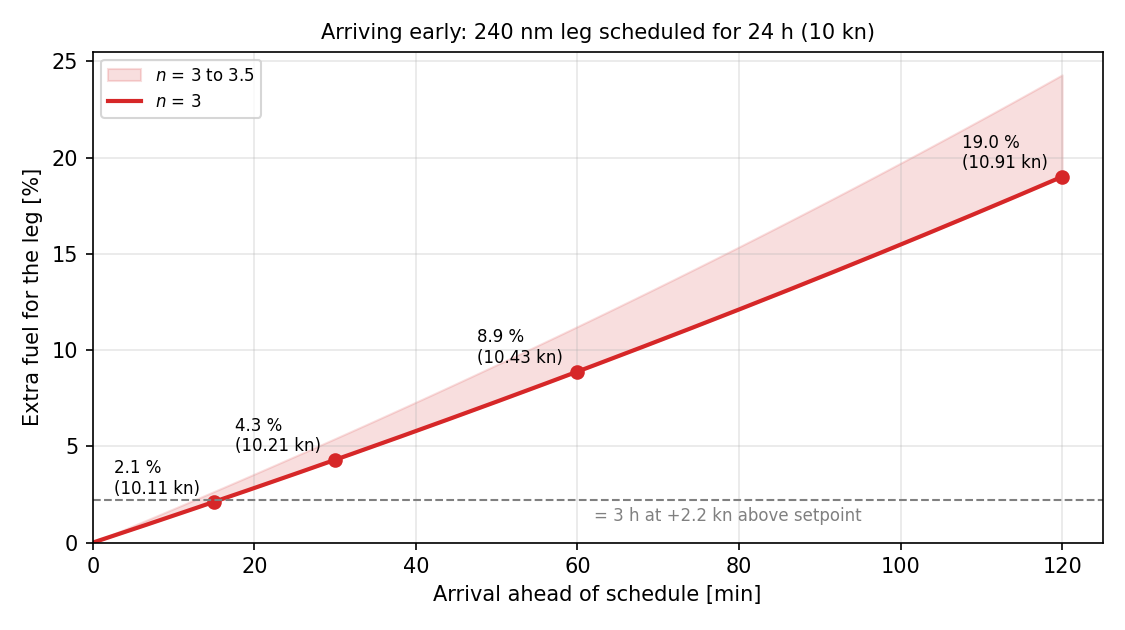
\includegraphics[width=0.8\textwidth]{images/early_arrival_penalty.png}
\caption{Extra fuel from arriving early, 240 nm leg scheduled for 24 h.  The band shows fuel rate exponents \(n\) = 3 to 3.5.}
\end{figure}

\begin{figure}[htbp]
\centering
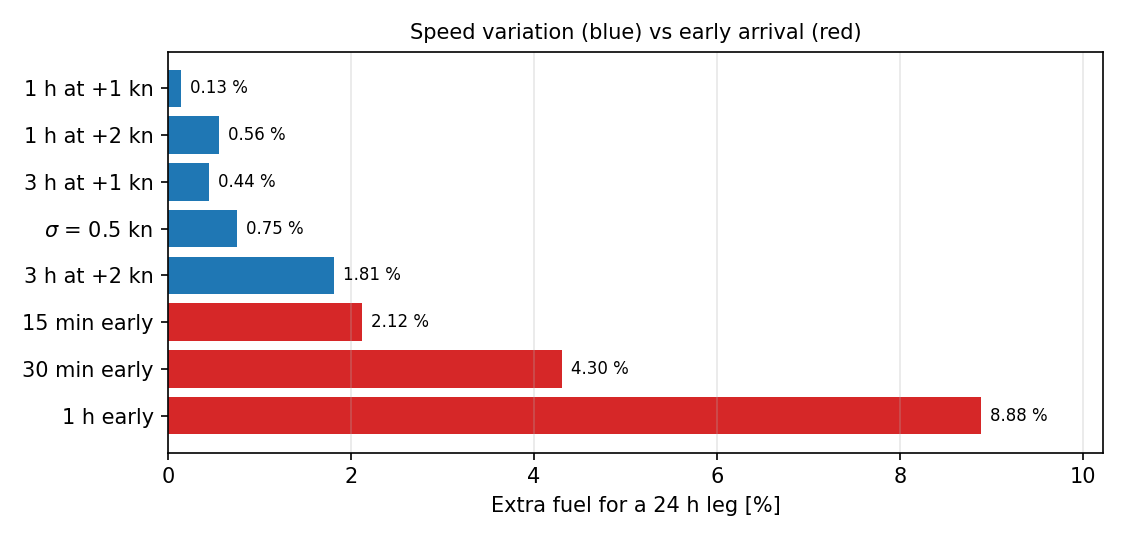
\includegraphics[width=0.8\textwidth]{images/speed_control_comparison.png}
\caption{Speed variation compared with early arrival, 24 h leg at 10 kn average.}
\end{figure}

\subsection{Interpretation}
\label{sec:orgf0a4c24}

\begin{itemize}
\item The main saving potential of speed control is not tighter speed
tracking, but the ability to sail at exactly the speed the schedule
requires, without a margin for drifting speed.
\item Rule of thumb: every 15 minutes of unnecessary arrival margin on a
24-hour leg costs about 2 \% fuel.  Every 0.1 kn of unnecessary speed
at 10 kn costs about 2 \%.
\item Part of the arrival margin covers real voyage uncertainty (weather,
pilot and berth times, tides).  Speed control removes the
speed-holding uncertainty, not the voyage uncertainty.
\item The saving depends on how the vessel was operated before.  It should
be documented per vessel from arrival times and average speeds before
and after installation.
\item On Link Galaxy the crew uses speed control more than 90 \% of the
transit time and holds the setpoint within ±0.1 kn.
\item A natural extension is an ETA hold function, where the speed setpoint
is calculated from distance to go and the required arrival time.
\end{itemize}

\section{Conclusions}
\label{sec:orgc5c0eea}

\begin{itemize}
\item With a fixed arrival time, a fuel cap gives no fuel saving compared
with speed control on this route (+0.1--0.2 \%), and a tight cap
compromises the schedule.
\item The fuel benefit the owner is looking for is better obtained by
planned speed: ETA hold, extended with current and weather forecasts.
With a Flettner rotor this is worth about 0.6 \% on this route.
\item The largest speed-related saving is to avoid sailing faster than the
schedule requires (Section 4): about 2 \% per 15 minutes of unnecessary
arrival margin on a 24 h leg.
\end{itemize}

\section{Data sources and acknowledgement}
\label{sec:orga0e87bb}

\begin{itemize}
\item This study has been conducted using E.U. Copernicus Marine Service
Information; \url{https://doi.org/10.48670/moi-00059}.  Product: Atlantic --
European North West Shelf -- Ocean Physics Reanalysis, product ID
\texttt{NWSHELF\_MULTIYEAR\_PHY\_004\_009}, dataset
\texttt{cmems\_mod\_nws\_phy-uv\_my\_7km-2D\_PT1H-i}.
\item Wave and wind data: NORA3 hindcast, Norwegian Meteorological Institute
(MET Norway), licensed under CC BY 4.0.
\end{itemize}
\end{document}
